\begin{center}
Problema E

Encontro na Final

{\tiny Por Márcio Belo}

Timelimit: $1$	
\end{center}			

No torneio esportivo Copa do Belo, as partidas são disputadas por dois participantes e são do tipo mata-mata, ou seja, o ganhador segue para a próxima fase, e o perdedor é eliminado da competição. 
O chaveamento do torneio é fixo e os participantes vencedores vão avançando nas chaves conhecidas até que haja dois times na final. 
O chaveamento do torneio é uma árvore binária de jogos onde as folhas são os times da competição. 
Os nós pais da árvore serão ocupados pelo time vencedor dentre os dois nós filhos. 
Entretanto, o número de participantes iniciais do torneio não necessariamente é uma potência de 2, por isso, no chaveamento, alguns times podem estar em uma fase anterior no início do torneio. 
Nesse caso, considere sempre o chaveamento em que a árvore está balanceada para a esquerda. 
Além disso, o chaveamento dos times é feito de forma aleatória para os nós folhas da árvore. 

O exemplo a seguir apresenta um chaveamento para $n=5$ times. Como não é potência de 2, o chaveamento fica desbalanceado para esquerda. 

\begin{center} 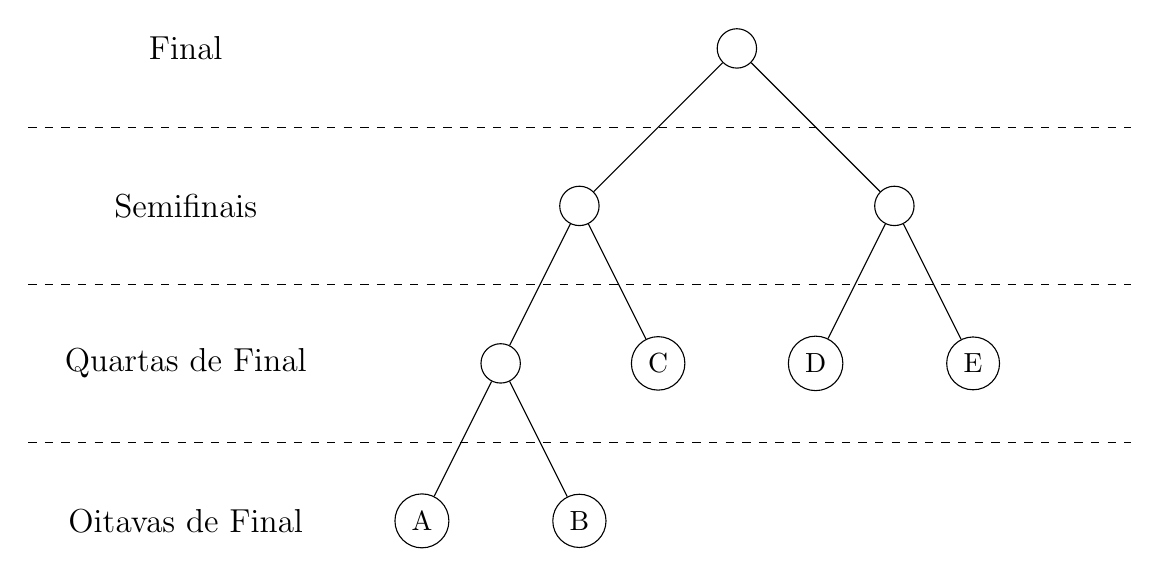
\begin{tikzpicture}
    % Nodes
    \node[draw, minimum size=5mm, circle] (A) at (0,0) {A};
    \node[draw, minimum size=5mm, circle] (B) at (2,0) {B};
    \node[draw, minimum size=5mm, circle] (AB) at (1,2) {};
    \node[draw, minimum size=5mm, circle] (C) at (3,2) {C};
    \node[draw, minimum size=5mm, circle] (D) at (5,2) {D};
    \node[draw, minimum size=5mm, circle] (E) at (7,2) {E};
    \node[draw, minimum size=5mm, circle] (ABC) at (2,4) {};
    \node[draw, minimum size=5mm, circle] (DE) at (6,4) {};
    \node[draw, minimum size=5mm, circle] (ABCDE) at (4,6) {};

    % Lines
    \draw[-] (A) -- (AB);
    \draw[-] (B) -- (AB);
    \draw[-] (AB) -- (ABC);
    \draw[-] (C) -- (ABC);
    \draw[-] (D) -- (DE);
    \draw[-] (E) -- (DE);
    \draw[-] (ABC) -- (ABCDE);
    \draw[-] (DE) -- (ABCDE);


    \node[] at (-3,6) {\large Final};
    \node[] at (-3,4) {\large Semifinais};
    \node[] at (-3,2) {\large Quartas de Final};
    \node[] at (-3,0) {\large Oitavas de Final};
    \draw [dashed] (-5,5) -- (9,5);
    \draw [dashed] (-5,3) -- (9,3);
    \draw [dashed] (-5,1) -- (9,1);
  
\end{tikzpicture} \end{center}

Para um chaveamento $n=7$ times, o chaveamento fica da seguinte forma 
\begin{center} 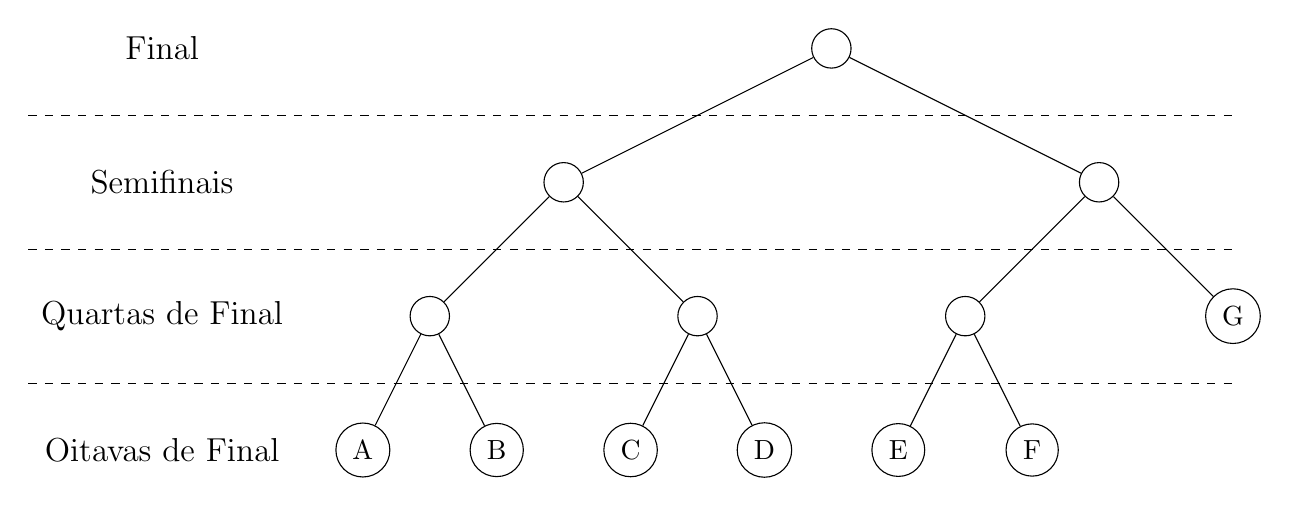
\begin{tikzpicture}[scale=0.85]
    % Nodes
    \node[draw, minimum size=5mm, circle] (8F1) at (0,0) {A};
    \node[draw, minimum size=5mm, circle] (8F2) at (2,0) {B};
    \node[draw, minimum size=5mm, circle] (8F3) at (4,0) {C};
    \node[draw, minimum size=5mm, circle] (8F4) at (6,0) {D};
    \node[draw, minimum size=5mm, circle] (8F5) at (8,0) {E};
    \node[draw, minimum size=5mm, circle] (8F6) at (10,0) {F};
    
    \node[draw, minimum size=5mm, circle] (4F1) at (1,2) {};
    \node[draw, minimum size=5mm, circle] (4F2) at (5,2) {};
    \node[draw, minimum size=5mm, circle] (4F3) at (9,2) {};
    \node[draw, minimum size=5mm, circle] (4F4) at (13,2) {G};
    
    \node[draw, minimum size=5mm, circle] (SF1) at (3,4) {};
    \node[draw, minimum size=5mm, circle] (SF2) at (11,4) {};
    
    \node[draw, minimum size=5mm, circle] (Final) at (7,6) {};

    % Lines
    \draw[-] (8F1) -- (4F1);
    \draw[-] (8F2) -- (4F1);
    \draw[-] (8F3) -- (4F2);
    \draw[-] (8F4) -- (4F2);
    \draw[-] (8F5) -- (4F3);
    \draw[-] (8F6) -- (4F3);
    
    \draw[-] (4F1) -- (SF1);
    \draw[-] (4F2) -- (SF1);
    \draw[-] (4F3) -- (SF2);
    \draw[-] (4F4) -- (SF2);

    \draw[-] (SF1) -- (Final);
    \draw[-] (SF2) -- (Final);

    \node[] at (-3,6) {\large Final};
    \node[] at (-3,4) {\large Semifinais};
    \node[] at (-3,2) {\large Quartas de Final};
    \node[] at (-3,0) {\large Oitavas de Final};
    \draw [dashed] (-5,5) -- (13,5);
    \draw [dashed] (-5,3) -- (13,3);
    \draw [dashed] (-5,1) -- (13,1);
  
\end{tikzpicture} \end{center}

O prof. Belo sabe que dois times são muito fortes e vão ganhar todos os seus jogos, e um encontro entre eles é esperado. A questão é, qual a probabilidade desses dois times se encontrarem na final da Copa do Belo? 


\vspace{0.3cm}
\textbf{Entrada}
Cada entrada contém uma única linha com o número $N$ de times, com $(2 \leq N \leq 10^{9})$. 

\vspace{0.3cm}
\textbf{Saída}
O sistema deve retornar a probabilidade de dois times que vencem todos os jogos se encontrarem na final. A probabilidade deve estar em porcentagem, com 3 casas decimais. Não é necessário imprimir o símbolo "\%". 

\begin{table}[h]
    \centering
    \begin{tabular}{|p{7cm}|p{7cm}|}
        \hline
        \begin{center}
            \vspace{-0.3cm}
            \textbf{Exemplos de Entrada}
            \vspace{-0.3cm}
        \end{center} 
         &  
        \begin{center}
            \vspace{-0.3cm}
            \textbf{Exemplos de Saída}
            \vspace{-0.3cm}
        \end{center} \\ \hline
         \texttt{2} & \texttt{100.000} \\  
         \hline
         \texttt{3} & \texttt{66.667} \\ 
         \hline
         \texttt{8} & \texttt{57.143} \\ 
         \hline
         \texttt{500} & \texttt{50.071} \\ 
         \hline
    \end{tabular}
    \caption{Exemplos de entradas e saídas}
    \label{tab:inputJ2}
\end{table}

\newpage

\begin{center}
\noindent
\lstinputlisting{abobora_23/E/E3.cpp}
\end{center}